\documentclass[UTF8,12pt,a4paper]{ctexart}

\usepackage{amsmath,amssymb}
\usepackage{booktabs}
\usepackage{geometry}
\usepackage{graphicx}
\usepackage[hidelinks]{hyperref}
\geometry{left=2.5cm,right=2.5cm,top=2.5cm,bottom=2.5cm}
\newcommand{\keywords}[1]{\par\noindent\textbf{关键词：}#1}

% 这是无官方 LaTeX 模板时的构建基线，不替代当届官方规则。
\title{微网典型日结果：导出链路样例}
\author{}
\date{}

\begin{document}
\maketitle

\begin{abstract}
本样例仅验证真实计算结果到图表、原生公式、中文 PDF 和资源记录的导出链路。典型日最优购电量为 59482.698167 kWh，购电费用为 35126.948941 元，期初与期末储能量均为 6000 kWh。本文件不是完整论文。
\keywords{微网；线性规划；储能；导出样例}
\end{abstract}

\clearpage
\section{典型日真实结果}
储能状态满足下式，充放电量定义在交流侧，时间步长为十分钟：
\begin{equation}
E_{t+1}=E_t+0.9x_t-y_t/0.9.
\end{equation}
图\ref{fig:q1-smoke}来自本项目真实典型日求解。表\ref{tab:smoke}列出实际计算汇总。
\begin{figure}[htbp]
\centering
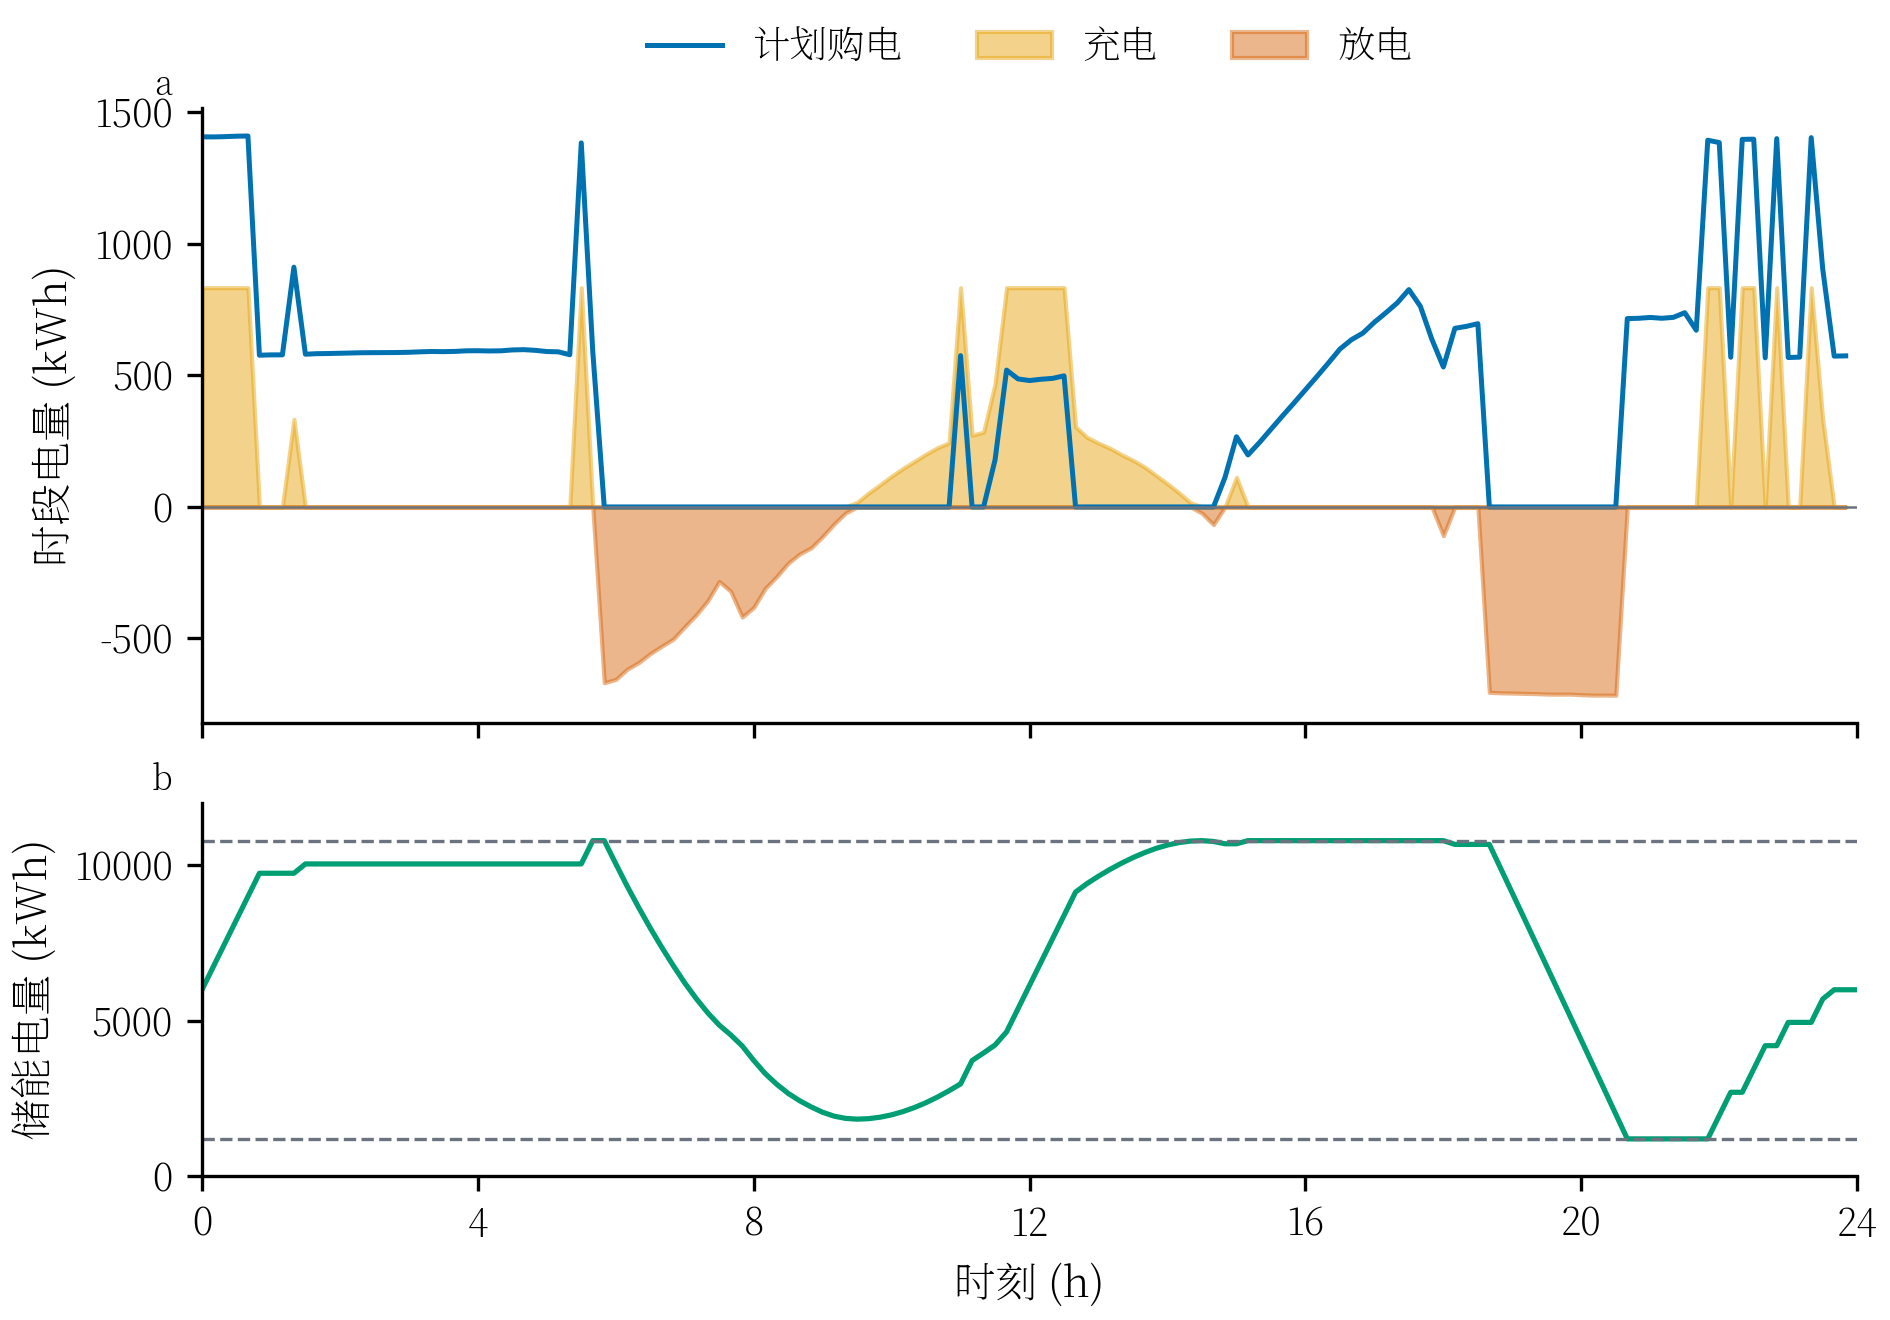
\includegraphics[width=0.90\linewidth]{figs/result_q1_optimal_schedule.png}
\caption{典型日购电、充放电与储能状态}
\label{fig:q1-smoke}
\end{figure}
\begin{table}[htbp]
\centering
\caption{典型日汇总}
\label{tab:smoke}
\begin{tabular}{lr}
\toprule 指标 & 数值 \\
\midrule 购电量（kWh） & 59482.698167 \\
购电费用（元） & 35126.948941 \\
期末储能量（kWh） & 6000 \\
\bottomrule
\end{tabular}
\end{table}
\end{document}
